\section{Uso avanzado de la Shell}

%-----------------------    ---------------------------------

\begin{frame}
\frametitle{Acortadores de teclado}

\begin{itemize}
   \item \texttt{Tab}: autocompleta programas, ficheros y directorios
   \item \texttt{Ctrl+A}: va al principio de la línea
   \item \texttt{Ctrl+E}: va al final de la línea
   \item \texttt{Ctrl+R}: busca por lo intrducido en la historia
   \item \texttt{Ctrl+K}: borra desde el punto actual al final
   \item \texttt{Ctrl+U}: borra hasta el punto actual
   \item \texttt{Ctrl+L}: \emph{aclara} la pantalla (como el mandato \texttt{clear})
   \item \texttt{Alt+F}: se mueve a la siguiente palabra
   \item \texttt{Alt+B}: se mueve a la palabra anterior
\end{itemize}

(algunos se pueden configurar en el propio terminal)


\end{frame}


%-----------------------    ---------------------------------

\begin{frame}
\frametitle{Uso de pestañas}

\begin{center}
  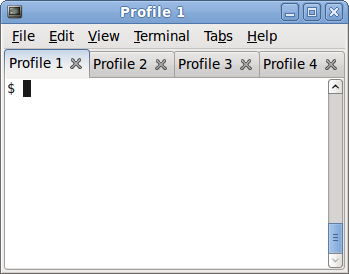
\includegraphics[width=4.5cm]{figs/tabs.png}
\end{center}


\begin{flushright}
{\tiny
http://unix.stackexchange.com/tags/gnome-terminal/info
}
\end{flushright}


\begin{itemize}
   \item Puedes poner nombre (título a cada pestaña)
   \item Nueva pestaña: \texttt{Ctrl+Alt+T} (yo lo suelo configurar como \texttt{Ctrl+T} para que sea igual que crear una nueva pestaña en el navegador)
   \item Pestaña siguiente/anterior: \texttt{Ctrl+PgUp} o \texttt{Ctrl+PgAbajo}
   \item \texttt{Alt+\emph{N}}: vas a la pestaña \emph{N}
\end{itemize}


\end{frame}


%-----------------------    ---------------------------------

\begin{frame}
\frametitle{Procesos}

\begin{itemize}
   \item \texttt{top}: Muestra los procesos según su \emph{consumo}
   \item \texttt{ps aux}: Lista todos los procesos del usuario
   \item \texttt{grep \emph{expr}}: Filtra por \emph{expr} 
   \item \texttt{ps aux | grep python}: Muestra la información de procesos que contengan \emph{python}
   \item \texttt{kill -9 \emph{pid}}: \emph{mata} el proceso con identificador \emph{pid}
\end{itemize}


\end{frame}


%-----------------------    ---------------------------------

\begin{frame}
\frametitle{Un pequeño chiste friqui para terminar}

\begin{center}
  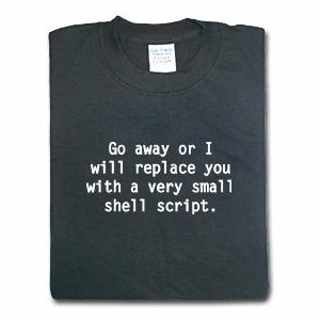
\includegraphics[width=7cm]{figs/shellscriptjoke.jpg}
\end{center}


\begin{flushright}
{\tiny
http://img819.imageshack.us/img819/4539/shellscriptjoke.jpg
}
\end{flushright}

\end{frame}

